%% Assignment #4 for disjoint set and breadth-first search

\documentclass[10pt,fullpage]{article}

\usepackage{amsmath,amssymb,amsthm,amsfonts} % Typical maths resource packages

%Check if we are compiling under latex or pdflatex
\ifx\pdftexversion\undefined
\usepackage[dvips]{graphicx}
%%%%%%%%
%% Pour inclure du .jpg et .pnm sous latex
%%%%%%%%%%%%%%
\DeclareGraphicsExtensions{.jpg,.eps,.pnm}
\DeclareGraphicsRule{.jpg}{eps}{.jpg.bb}{`jpeg2ps -h #1}
\DeclareGraphicsRule{.pnm}{eps}{.pnm.bb}{`pnmtops #1} \else
\usepackage[pdftex]{graphicx}
\fi

\usepackage{hyperref}                 % For creating hyperlinks in cross references

\usepackage{listings}

\usepackage{qtree}

\topmargin -1.5cm \oddsidemargin -0.04cm \evensidemargin -0.04cm
\textwidth 16.00cm \textheight 23.50cm
\parskip 7.2pt
\parindent 0.25in

\makeindex

\title{ Advanced Algorithms Assignment IV }


\author{Matthew Bennett \\
{\small\em Too much HW: Disjoint Set and Breadth-First Search\ Draft
date \today }}

 \date{ }

\begin{document}
\maketitle

\textbf{Exercises 21.1-1 Suppose that CONNECTED-COMPONENTS is run on
the undirected graph G = (V, E), where V = {a, b, c, d, e, f, g, h,
i, j, k} and the edges of E are processed in the following order:
(d, i), (f, k), (g, i), (b, g), (a, h), (i, j), (d, k), (b, j), (d,
f), (g, j), (a, e), (i, d). List the vertices in each connected
component after each iteration of lines 3-5. }
\begin{tabbing}
CONNECTED-COMPONENTS(G)\\
1 for \= each \= vertex v $\epsilon$ V[G]\\
2 \> do MAKE-SET(v)\\
3 for each edge (u, v) $\epsilon$ E[G]\\
4 \> do if FIND-SET(u) $\neq$ FIND-SET(v)\\
5 \> \> then UNION(u, v)\\
\end{tabbing}

\begin{tabular}{|r|r|r|r|r|r|r|r|r|r|r|r|r|}
  \hline
  Init. & \{a\} & \{b\} & \{c\} & \{d\} & \{e\} & \{f\} & \{g\} & \{h\} & \{i\} & \{j\} & \{k\} \\
  (d,i) & \{a\} & \{b\} & \{c\} & \{d,i\} & \{e\} & \{f\} & \{g\} & \{h\} &  & \{j\} & \{k\} \\
  (f,k) & \{a\} & \{b\} & \{c\} & \{d,i\} & \{e\} & \{f,k\} & \{g\} & \{h\} &  & \{j\} &  \\
  (g,i) & \{a\} & \{b\} & \{c\} & \{d,g,i\} & \{e\} & \{f,k\} & & \{h\} &  & \{j\} &  \\
  (b,g) & \{a\} & \{b,d,g,i\} & \{c\} & & \{e\} & \{f,k\} & & \{h\} &  & \{j\} &  \\
  (a,h) & \{a,h\} & \{b,d,g,i\} & \{c\} & & \{e\} & \{f,k\} & & &  & \{j\} &  \\
  (i,j) & \{a,h\} & \{b,d,g,i,j\} & \{c\} & & \{e\} & \{f,k\} & & &  & &  \\
  (d,k) & \{a,h\} & \{b,d,f,g,i,j,k\} & \{c\} & & \{e\} & & & &  & &  \\
  (b,j) & \{a,h\} & \{b,d,f,g,i,j,k\} & \{c\} & & \{e\} & & & &  & &  \\
  (d,f) & \{a,h\} & \{b,d,f,g,i,j,k\} & \{c\} & & \{e\} & & & &  & &  \\
  (g,j) & \{a,h\} & \{b,d,f,g,i,j,k\} & \{c\} & & \{e\} & & & &  & &  \\
  (a,e) & \{a,e,h\} & \{b,d,f,g,i,j,k\} & \{c\} & & & & & &  & &  \\
  (i,d) & \{a,e,h\} & \{b,d,f,g,i,j,k\} & \{c\} & & & & & &  & &  \\
  \hline
\end{tabular}


\newpage

\textbf{Exercises 21.1-3 During the execution of
CONNECTED-COMPONENTS on an undirected graph $G = (V, E)$ with k
connected components, how many times is FIND-SET called? How many
times is UNION called? Express your answers in terms of $|V|$,
$|E|$, and $k$.]}

\begin{tabbing}
CONNECTED-COMPONENTS(G)\\
1 for \= each \= vertex v $\epsilon$ V[G]\\
2 \> do MAKE-SET(v)\\
3 for each edge (u, v) $\epsilon$ E[G]\\
4 \> do if FIND-SET(u) $\neq$ FIND-SET(v)\\
5 \> \> then UNION(u, v)\\
\end{tabbing}

The only time FIND-SET is called is twice for each edge, which is a
constant. FIND-SET is run $2|E| = \Theta(|E|)$ times.\\

UNION is called whenever an edge $(u,v)$ has vertices u, v in
disjoint sets. That is, UNION(u,v) is only invoked whenever no edges
from the set U and the set V have been investigated. If we let $k =
|V|$, then Union must be called $|V|$ times, because the total
number of disjoint sets will also be $|V|$, and the graph is a fully
connected mesh. If $k = 0$, the for loop of line (3) will not run
because $|E| = 0$.\\

Each time that Union is called, it reduces the total number of
disjoint sets available. It is clear that UNION must run at least k
times, since k components of the graph are connected. The complete
mesh uses $|V|$ calls. Each call to UNION removes 1 disjoint set.
Therefore, the number of UNION calls should be $|V| - k =
\Theta(|V|)$.

\newpage

\textbf{Exercises 21.2-2  Show the data structure that results and
the answers returned by the FIND-SET operations in the following
program. Use the linked-list representation with the weighted-union
heuristic. Assume that if the sets containing $x_i$ and $x_j$ have
the same size, then the operation UNION$(x_i, x_j)$ appends $x_j$'s
list onto $x_i$'s list.}\\
 1  for i = 1 to 16      do MAKE-SET($x_i$)\\
 2  for i = 1 to 15 by 2 do UNION($x_i, x_{i+1}$)\\
 3  for i = 3 to 11 by 4 do UNION($x_i, x_{i+3}$)\\
 4  UNION($x_2, x_{14}$)\\
 5  UNION($x_6, x_2$)\\
 6  FIND-SET($x_3$)\\
 7  FIND-SET($x_{10}$)\\\\

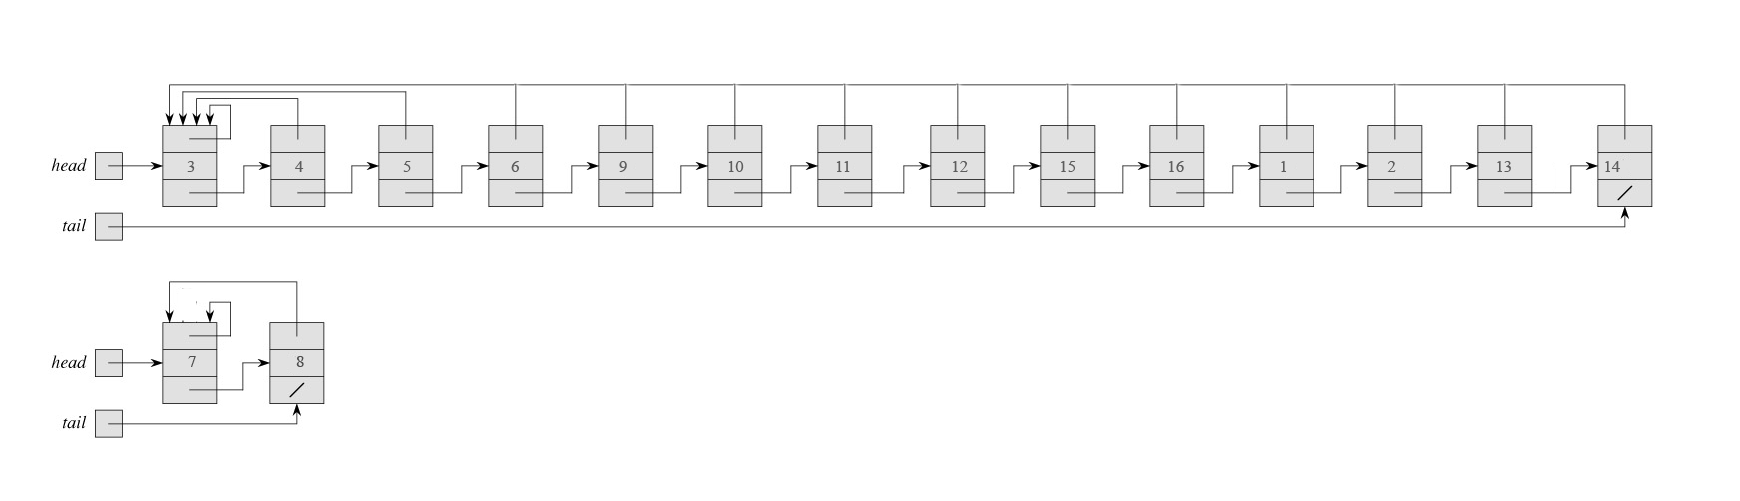
\includegraphics{21_2.png}


\newpage

\textbf{Exercises 22.1-1 Given an adjacency-list representation of a
directed graph, how long does it take to compute the out-degree of
every vertex? How long does it take to compute the in-degrees?}

The out-degree of a single vertex is found by counting the number of
links in its adjacency list, which a constant, at most $|E|$ or
$|V|$. The adjacency list for such a vertex can be retrieved in a
constant amount of time (think hash table). So the out degree of a
single vertex can be computed in $O(|V| + |E|)$ time, and the out
degree for every single vertex can be done in $O(|V||E|)$ time.\\

The in-degree of a single vertex is found by traversing the total
number of adjacency lists, $|V|$, which each have at most $|E|$
links, a constant. So the total time needed to find the in-degree of
a single vertex is $O(|V| + |E|)$. To compute the in-degree of every single vertex requires O(|V||E|) time. \\

I was a little confused about what "every vertex" meant. Does it
mean All vertices, or Each vertex (the efficiency being same)? I
gave both answers to appease the Corman, Leiserson, Rivest Gods.

\newpage

\textbf{Exercises 22.1-2 Give an adjacency-list representation for a
complete binary tree on 7 vertices. Give an equivalent
adjacency-matrix representation. Assume that vertices are numbered
from 1 to 7 as in a binary heap.}

I used the min-heap numbering scheme. I.E.: 1 is the root, 2-3 are
intermediate nodes, and 4-7 are all leaves. Also, the tree is singley-linked\\

Adjacency list:\\
$1\rightarrow2\rightarrow3$\\
$2\rightarrow4\rightarrow5$\\
$3\rightarrow6\rightarrow7$\\
$4\rightarrow$\\
$5\rightarrow$\\
$6\rightarrow$\\
$7\rightarrow$\\

Adjacency Matrix:\\
$\left(
  \begin{array}{ccccccc}
    0 & 1 & 1 & 0 & 0 & 0 & 0 \\
    0 & 0 & 0 & 1 & 1 & 0 & 0 \\
    0 & 0 & 0 & 0 & 0 & 1 & 1 \\
    0 & 0 & 0 & 0 & 0 & 0 & 0 \\
    0 & 0 & 0 & 0 & 0 & 0 & 0 \\
    0 & 0 & 0 & 0 & 0 & 0 & 0 \\
    0 & 0 & 0 & 0 & 0 & 0 & 0 \\
  \end{array}
\right)$

\newpage

\textbf{Exercises 22.2-2 Show the $d$ and $\pi$ values that result
from running breadth-first search on the undirected graph of Figure
22.3, using vertex u as the source.}

Yay, I did this one for HW in the first Algorithms class. Let me see
here ...

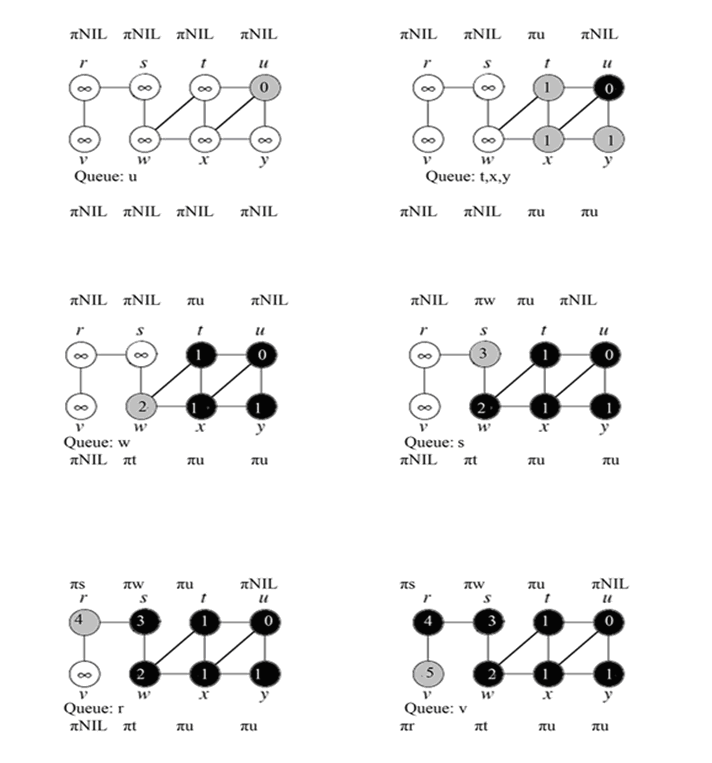
\includegraphics[scale=0.5]{22_2.png}

\newpage

\textbf{Exercises 22.2-3 What is the running time of BFS if its
input graph is represented by an adjacency matrix and the algorithm
is modified to handle this form of input?}

\begin{verbatim}for each v in Adj[u]  (1)\end{verbatim}

$O(|V|^2)$, since (1) must be changed to a nested-for to visit all
rows and cols of the adjacency matrix--$|V|^2$ of them

\newpage

\textbf{Exercises 22.2-6  There are two types of professional
wrestlers: "good guys" and "bad guys." Between any pair of
professional wrestlers, there may or may not be a rivalry. Suppose
we have n professional wrestlers and we have a list of r pairs of
wrestlers for which there are rivalries. Give an O($n + r$)-time
algorithm that determines whether it is possible to designate some
of the wrestlers as good guys and the remainder as bad guys such
that each rivalry is between a good guy and a bad guy. If is it
possible to perform such a designation, your algorithm should
produce it. }

Hrmm. I think we did this last semester as well, but I can't find my
solution. Here goes:\\

Start with a graph, where all the wrestlers are vertices, and the
rivalries are edges. Don't worry about which wrestlers are good-guys
and which are bad guys, yet. Perform a breadth-first search starting
anywhere. After the search has completed, mark the root node of the
BFS as either a good guy or bad guy. Whichever label you choose is
entirely subjective, but will affect the result of the algorithm.
Mark the rest of the wrestlers depending on their BFS distance. Even
numbers inherit the root's marking, and odd numbers get labeled
whatever the root is not.\\

Wrestlers who are infinitely far away in the BFS can be marked good
or bad with no consequence to the root node, but the graphs they are
associated with must also have a BFS performed and the same labeling
method applied. Finally, if there are any odd-length cycles in the
rivalry graphs, a bipartite labeling cannot be performed. The
absolute concept of good and bad doesn't apply here--Nietzsche would
be upset.\\

The algorithm uses two steps. The BFS is $O(n)$ (number of
vertices), but the labels might not be valid if the graph is not
bi-partite (has an odd-length cycle). Therefore, we must check and
make sure all edges connect a good guy to a bad guy, which takes
$O(r)$ time (number of edges). Therefore the total run time for the
algorithm should be $O(n + r)$, as specified.\\

Phew.\\

\newpage

\end{document}
